\chapter{Desenvolvimento vegetativo das plantas: meristemas e crescimento}\label{ch:b2:plant-meristems}

Um carvalho que era uma plântula quando a catedral foi construída
ainda acrescenta um anel de \omterm{def:b2:plant-meristems:wood}{madeira} a cada ano, ainda abre folhas novas
a cada primavera, ainda empurra novas pontas de raiz pelo solo. Nenhum
animal faz isso; um cavalo para de crescer aos quatro anos. A diferença
é que uma planta conserva, na ponta de cada caule e de cada raiz e num
fino cilindro dentro de cada tronco, pequenas populações de células
embrionárias --- os \emph{\omterm{def:b2:plant-meristems:meristem}{meristemas}} --- que nunca param de se dividir
e que constroem o corpo da planta para fora e para cima enquanto ela
viver. Este capítulo examina como os dois \omterm{def:b2:plant-meristems:meristem}{meristemas} apicais são
organizados e controlados, como uma célula vegetal cresce, como os
hormônios decidem a forma de um caule e como um tronco engrossa.

\section{Os meristemas}

\begin{definition}[Os meristemas e os dois tipos de crescimento]\label{def:b2:plant-meristems:meristem}
\index{meristema}\index{meristema apical caulinar}\index{meristema apical radicular}\index{câmbio}
Um \emph{meristema} é uma população de células pequenas,
indiferenciadas e em divisão, que persiste por toda a vida da planta e
da qual derivam todos os seus tecidos. O \emph{meristema apical
caulinar} (MAC), na ponta de cada caule, forma as folhas, o caule e, na
estação, as \omterm{def:b2:angiosperm-reproduction:flower}{flores}; o \emph{meristema apical radicular} (MAR), atrás de
cada ponta de raiz, forma a raiz; juntos, eles comandam o
\emph{crescimento primário}, o alongamento da planta. Os
\emph{meristemas laterais} --- o \emph{\omterm{def:b2:plant-meristems:wood}{câmbio vascular}} e o
\emph{felogênio}, finos cilindros dentro dos caules e das raízes ---
comandam o \emph{crescimento secundário}, o espessamento que forma a
\omterm{def:b2:plant-meristems:wood}{madeira} e a \omterm{def:b2:plant-meristems:wood}{casca}. O crescimento vegetal é, portanto,
\emph{indeterminado}: os meristemas podem continuar indefinidamente, e
a planta é um organismo modular, que repete a unidade
folha--nó--entrenó--gema enquanto as condições o permitirem. Toda gema
axilar é um MAC dormente, de modo que uma planta leva milhares de
pontos de crescimento de reserva.
\end{definition}

\begin{proposition}[O ápice caulinar]\label{prop:b2:plant-meristems:sam}
\index{filotaxia}\index{primórdio foliar}\index{plastocrono}
O MAC é um domo de um décimo de milímetro de diâmetro, com algumas
centenas de células. Suas uma ou duas camadas externas (a
\emph{túnica}) só se dividem no plano da superfície e dão a epiderme; a
massa abaixo delas (o \emph{corpo}) se divide em todos os planos. No
cume, uma \emph{zona central} de \omterm{def:b2:cell-differentiation:differentiation}{células-tronco} de divisão lenta
abastece uma \emph{zona periférica} de células de divisão mais rápida,
onde os \emph{\omterm{prop:b2:plant-meristems:sam}{primórdios foliares}} surgem como saliências a intervalos
regulares de tempo (o \emph{plastocrono}, de horas a dias) e a ângulos
regulares em torno do domo (a \emph{filotaxia}: oposta, verticilada ou
espiral segundo o ângulo áureo de \qty{137.5}{\degree}, que coloca cada
folha nova na maior lacuna deixada pelas outras). Abaixo, uma
\emph{zona medular} forma a medula e alonga o caule. Um primórdio se
forma onde o hormônio auxina se acumula na camada superficial e, à
medida que cresce, drena a auxina de seus arredores, e é por isso que o
primórdio seguinte surge o mais longe possível dele: o padrão se
auto-organiza.
\end{proposition}

\begin{omfigure}
\begin{tikzpicture}[every node/.style={font=\scriptsize}]
  % dome
  \draw[thick, fill=omExo!12] (-2.2,0) .. controls (-2.2,1.6) and (-0.8,2.6) .. (0,2.6) .. controls (0.8,2.6) and (2.2,1.6) .. (2.2,0) -- (2.2,-1.4) -- (-2.2,-1.4) -- cycle;
  % tunica layers
  \draw[thick, omDef] (-2.2,0) .. controls (-2.2,1.5) and (-0.8,2.45) .. (0,2.45) .. controls (0.8,2.45) and (2.2,1.5) .. (2.2,0);
  \draw[thick, omDef] (-2.05,0) .. controls (-2.05,1.35) and (-0.75,2.3) .. (0,2.3) .. controls (0.75,2.3) and (2.05,1.35) .. (2.05,0);
  % zones
  \draw[thick, dashed, omThm, fill=omThm!15] (0,1.75) ellipse (0.6 and 0.55);
  \draw[thick, dashed, omProp] (0,0.9) ellipse (1.6 and 1.35);
  \draw[thick, dashed, omExo!70!black] (-0.9,-0.9) rectangle (0.9,-0.1);
  % primordia
  \draw[thick, fill=omExo!40] (-2.2,0.4) .. controls (-2.5,1.4) and (-1.6,1.9) .. (-1.55,1.3) .. controls (-1.5,0.9) and (-1.9,0.6) .. (-2.2,0.4);
  \draw[thick, fill=omExo!40] (2.2,0.2) .. controls (2.7,1.0) and (2.1,1.5) .. (1.75,1.1) .. controls (1.6,0.8) and (1.9,0.5) .. (2.2,0.2);
  % labels
  \draw (0.4,2.1) -- (3.2,2.6) node[right, align=left] {zona central:\\células-tronco de divisão lenta};
  \draw (1.3,0.5) -- (3.2,1.4) node[right, align=left] {zona periférica:\\divisão rápida, primórdios foliares};
  \draw (0.6,-0.5) -- (3.2,0.0) node[right, align=left] {zona medular: medula,\\alongamento do caule};
  \draw (-1.7,1.5) -- (-3.0,2.4) node[left, align=right] {primórdio\\foliar};
  \draw (-1.2,2.05) -- (-3.0,1.2) node[left, align=right] {túnica: só divisões\\na superfície};
  \draw (2.2,0.7) -- (3.2,-1.0) node[right, align=left] {próximo primórdio,\\a \qty{137.5}{\degree}};
\end{tikzpicture}

{\small O \omterm{def:b2:plant-meristems:meristem}{meristema apical caulinar} em corte: uma túnica de uma ou duas
camadas superficiais sobre um corpo, uma zona central de \omterm{def:b2:cell-differentiation:differentiation}{células-tronco}
no cume, uma zona periférica onde os \omterm{prop:b2:plant-meristems:sam}{primórdios foliares} se projetam e
uma zona medular abaixo.}
\end{omfigure}

\begin{omfigure}
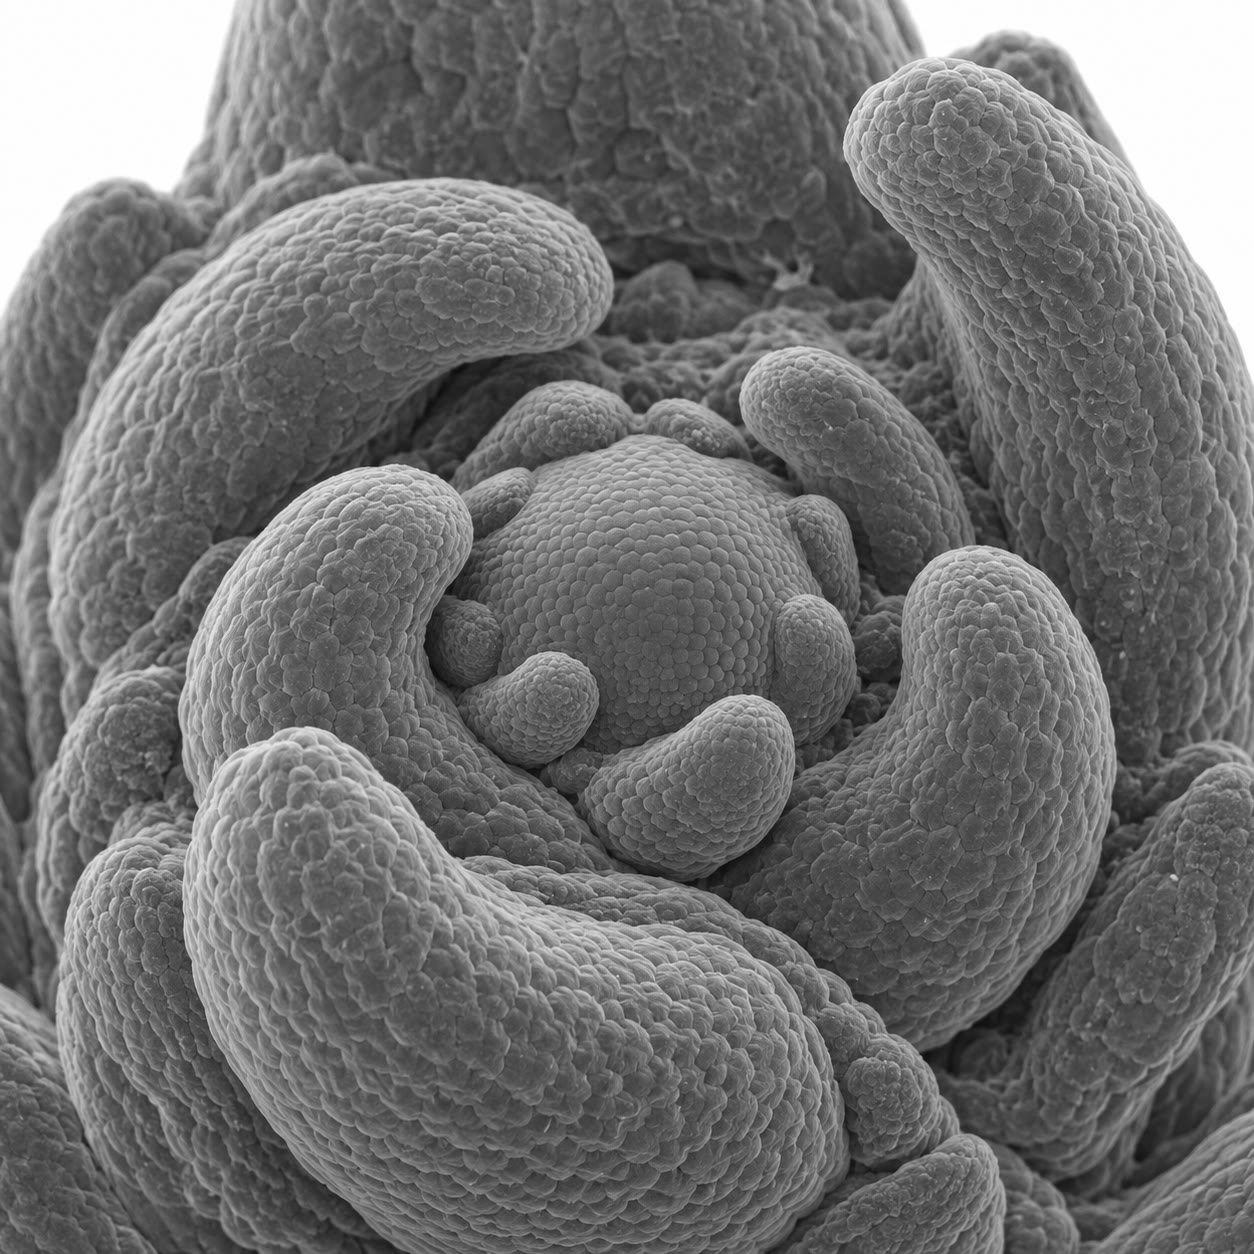
\includegraphics[width=0.44\linewidth]{images/book4/ai/b4-13-shoot-apex-sem.jpg}

{\small Um ápice caulinar ao microscópio eletrônico de varredura: o
domo liso do \omterm{def:b2:plant-meristems:meristem}{meristema} e a espiral de \omterm{prop:b2:plant-meristems:sam}{primórdios foliares} em torno
dele, cada novo primórdio colocado na lacuna mais larga.}
\end{omfigure}

\begin{proposition}[Manter as células-tronco: uma alça de retroalimentação]\label{prop:b2:plant-meristems:wus}
\index{WUSCHEL}\index{CLAVATA}\index{retroalimentação negativa!meristema}
O tamanho do estoque de \omterm{def:b2:cell-differentiation:differentiation}{células-tronco} é mantido constante por uma alça
entre dois genes. As células logo abaixo da zona central expressam o
\omterm{prop:b2:cell-differentiation:transcriptional}{fator de transcrição} \emph{WUSCHEL} (WUS), cujo produto sobe para as
células situadas acima e as mantém como \omterm{def:b2:cell-differentiation:differentiation}{células-tronco}; as
\omterm{def:b2:cell-differentiation:differentiation}{células-tronco}, por sua vez, secretam um pequeno peptídeo, o
\emph{CLAVATA3} (CLV3), que se difunde para baixo, liga-se a um
receptor-quinase (CLV1) nas células que expressam WUS e reprime o WUS.
Mais \omterm{def:b2:cell-differentiation:differentiation}{células-tronco} significam mais CLV3, menos WUS, menos
\omterm{def:b2:cell-differentiation:differentiation}{células-tronco}; menos \omterm{def:b2:cell-differentiation:differentiation}{células-tronco} significam menos CLV3, mais WUS,
mais \omterm{def:b2:cell-differentiation:differentiation}{células-tronco}. O estoque é, assim, uma quantidade regulada, como
as gonadotrofinas do \cref{ch:b2:reproductive-hormones}, e a mesma lógica --- um sinal da
população regulada que reprime o fator que a produz --- mantém também o
\omterm{def:b2:plant-meristems:meristem}{meristema} da raiz.
\end{proposition}
\begin{proof}[Evidências]
Os mutantes \emph{clavata} de Arabidopsis (Clark, Meyerowitz, década de
1990) têm \omterm{def:b2:plant-meristems:meristem}{meristemas} que incham até muitas vezes o tamanho normal, com
folhas extras, órgãos florais extras e caules fasciados (achatados, em
forma de fita): o freio desapareceu. Os mutantes \emph{wuschel} formam
um \omterm{def:b2:plant-meristems:meristem}{meristema} que para após algumas folhas e depois forma novos
\omterm{def:b2:plant-meristems:meristem}{meristemas}, cada um dos quais para por sua vez: o acelerador
desapareceu. No duplo mutante, o \omterm{def:b2:meiosis-heredity:vocabulary}{fenótipo} \emph{wuschel} prevalece, o
que coloca o WUS a jusante do CLV; e o peptídeo CLV3 aplicado a um
ápice selvagem reprime o WUS em poucas horas.
\end{proof}

\begin{proposition}[O ápice radicular]\label{prop:b2:plant-meristems:ram}
\index{coifa}\index{centro quiescente}\index{zona de alongamento}\index{pelo radicular}
Uma raiz cresce a partir de um \omterm{def:b2:plant-meristems:meristem}{meristema} abrigado atrás de uma
\emph{coifa}, cujas células se desprendem à medida que a ponta avança
pelo solo e que secreta uma mucilagem lubrificante e percebe a
gravidade (grãos de amido que sedimentam em suas células). No centro do
\omterm{def:b2:plant-meristems:meristem}{meristema}, um \emph{\omterm{prop:b2:plant-meristems:ram}{centro quiescente}} de algumas centenas de células
só se divide raramente; ele mantém as iniciais que o cercam --- da
coifa, da epiderme, do córtex e do cilindro vascular --- como
\omterm{def:b2:cell-differentiation:differentiation}{células-tronco}, mais ou menos como o WUS mantém as do caule. Atrás do
\omterm{def:b2:plant-meristems:meristem}{meristema} vem a \emph{\omterm{prop:b2:plant-meristems:ram}{zona de alongamento}}, alguns milímetros em que as
células se alongam de dez a vinte vezes, empurrando a ponta para a
frente; depois a \emph{zona de \omterm{def:b2:cell-differentiation:differentiation}{diferenciação}}, onde a epiderme forma os
\emph{\omterm{prop:b2:plant-meristems:ram}{pelos radiculares}} e o xilema e o floema amadurecem. As raízes
laterais não surgem na ponta, mas a partir do periciclo, no interior da
raiz madura, em frente aos polos do xilema, e abrem caminho através do
córtex. A auxina, produzida no caule e levada para baixo, acumula-se na
ponta e organiza todo o arranjo; o \omterm{prop:b2:plant-meristems:ram}{centro quiescente} fica em seu
máximo.
\end{proposition}

\begin{omfigure}
\begin{tikzpicture}[every node/.style={font=\scriptsize}]
  % root outline
  \draw[thick, fill=omExo!10] (-1.0,4.5) -- (-1.0,0.6) .. controls (-1.0,-0.4) and (1.0,-0.4) .. (1.0,0.6) -- (1.0,4.5);
  % root cap
  \draw[thick, fill=omExo!45] (-0.9,0.8) .. controls (-1.1,-0.1) and (1.1,-0.1) .. (0.9,0.8) .. controls (0.5,0.4) and (-0.5,0.4) .. (-0.9,0.8);
  % meristem
  \fill[omThm!25] (-0.85,0.8) rectangle (0.85,1.7);
  \fill[omThm!70] (0,0.95) ellipse (0.25 and 0.12);
  % elongation zone
  \fill[omProp!20] (-0.85,1.7) rectangle (0.85,3.0);
  % differentiation zone with root hairs and vascular strand
  \fill[omDef!15] (-0.85,3.0) rectangle (0.85,4.5);
  \fill[omDef!50] (-0.15,3.0) rectangle (0.15,4.5);
  \foreach \y in {3.2,3.5,3.8,4.1,4.4} { \draw[omDef!80!black] (1.0,\y) -- (1.7,\y+0.1); \draw[omDef!80!black] (-1.0,\y) -- (-1.7,\y+0.1); }
  % lateral root primordium
  \draw[thick, fill=omThm!30] (0.15,4.0) .. controls (0.5,3.9) and (0.8,4.1) .. (0.9,4.3) .. controls (0.7,4.35) and (0.4,4.3) .. (0.15,4.3);
  % labels
  \draw (0.5,0.4) -- (2.2,0.2) node[right] {coifa};
  \draw (0.25,0.95) -- (2.2,0.9) node[right] {centro quiescente};
  \draw (0.85,1.4) -- (2.2,1.5) node[right] {meristema (divisão)};
  \draw (0.85,2.4) -- (2.2,2.3) node[right, align=left] {zona de alongamento:\\as células se alongam $10\times$};
  \draw (1.5,3.6) -- (2.2,3.4) node[right] {pelos radiculares};
  \draw (0.0,4.2) -- (2.2,4.2) node[right] {cilindro vascular};
  \draw (0.7,4.3) -- (2.2,4.9) node[right, align=left] {primórdio de raiz lateral\\(a partir do periciclo)};
  \draw[->, thick] (-2.4,4.5) -- (-2.4,0.6); \node[left, rotate=90, anchor=south] at (-2.5,2.5) {a auxina flui para a ponta};
\end{tikzpicture}

{\small A ponta da raiz: coifa, \omterm{def:b2:plant-meristems:meristem}{meristema} com seu \omterm{prop:b2:plant-meristems:ram}{centro quiescente},
\omterm{prop:b2:plant-meristems:ram}{zona de alongamento} e zona de \omterm{def:b2:cell-differentiation:differentiation}{diferenciação}, com \omterm{prop:b2:plant-meristems:ram}{pelos radiculares} e
vasos maduros. As raízes laterais começam no interior, a partir do
periciclo.}
\end{omfigure}

\begin{omfigure}
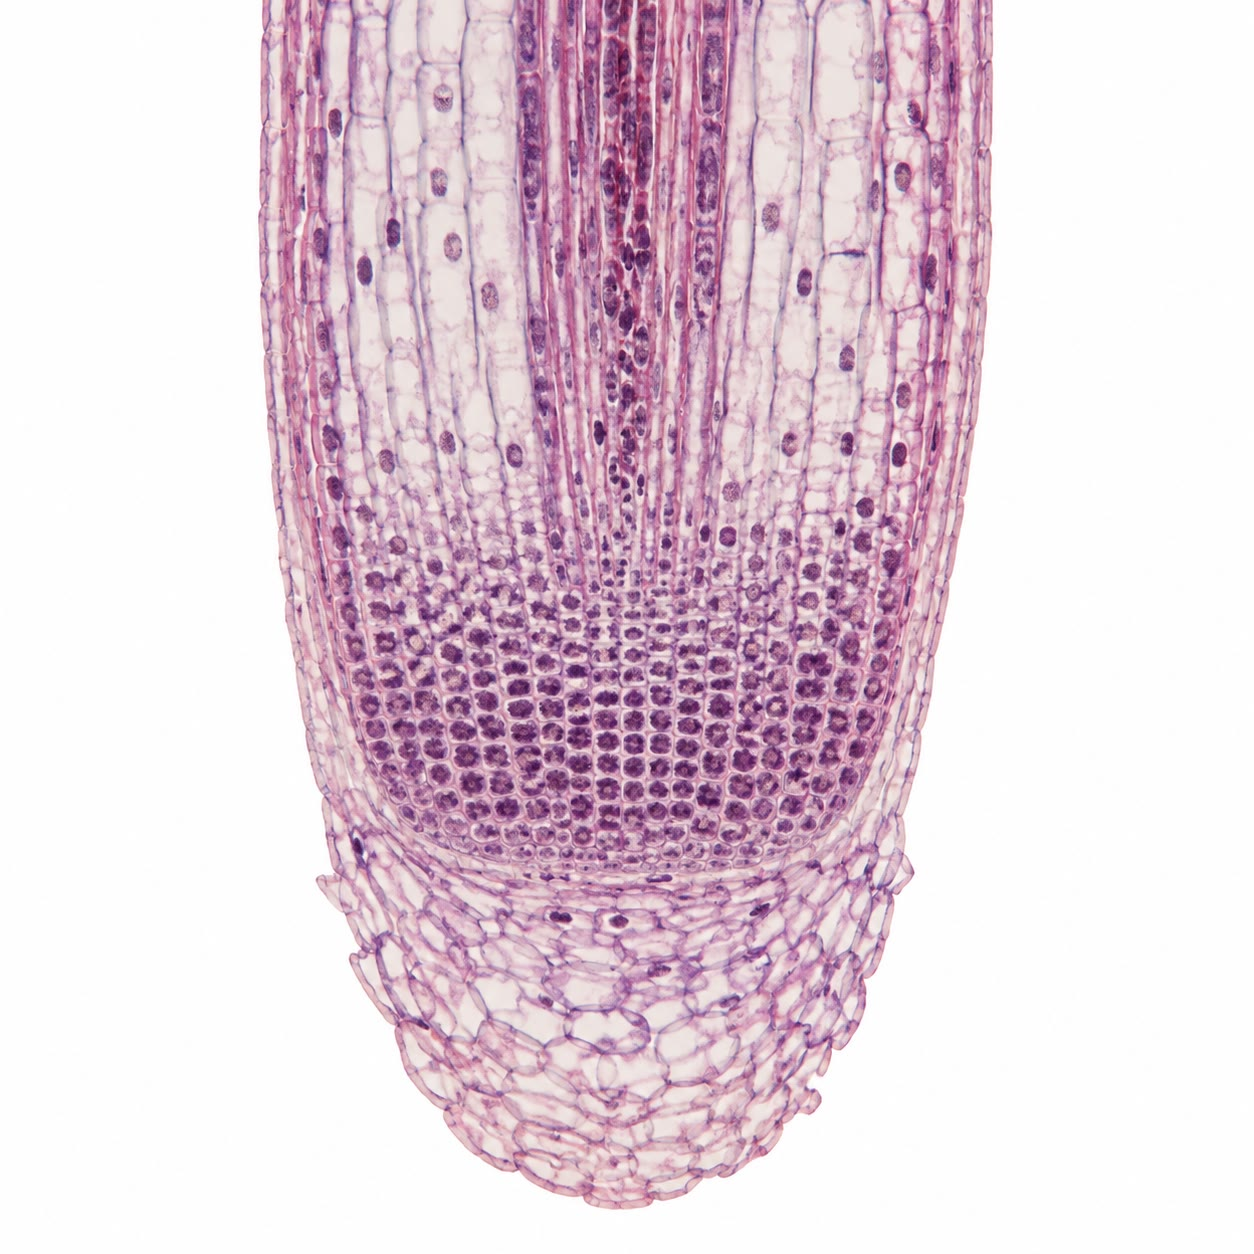
\includegraphics[width=0.42\linewidth]{images/book4/ai/b4-13-root-tip.jpg}

{\small Uma ponta de raiz em corte longitudinal: as células soltas da
coifa, o \omterm{def:b2:plant-meristems:meristem}{meristema} denso com seus núcleos escuros e as células em
alongamento acima.}
\end{omfigure}

\section{Como uma célula vegetal cresce}

\begin{theorem}[A equação de Lockhart]\label{thm:b2:plant-meristems:lockhart}
\index{turgescência}\index{parede celular!extensibilidade}\index{equação de Lockhart}
Uma célula vegetal cresce esticando sua parede sob a pressão de seu
próprio conteúdo. A parede só cede de forma irreversível acima de uma
turgescência limiar $Y$, e então a uma taxa proporcional ao excesso: a
taxa de crescimento relativo de uma célula de comprimento $L$ é
\[
\frac{1}{L}\frac{\mathrm{d}L}{\mathrm{d}t} = \phi\,(P - Y) \quad (P > Y),
\]
em que $P$ é a pressão de turgescência e $\phi$ a
\emph{extensibilidade} da parede. O crescimento é, portanto,
controlado por dois lados: pela água, que fixa $P$ (uma célula murcha
para de crescer), e pela parede, que fixa $\phi$ e $Y$ --- e é sobre a
parede que os hormônios agem. A auxina faz as células bombearem
prótons para a parede; a acidez ativa as \emph{expansinas}, proteínas
que afrouxam as ligações entre as fibrilas de celulose e a matriz,
elevando $\phi$ e reduzindo $Y$ em poucos minutos (\emph{crescimento
ácido}). Com $\phi =
\qty{0.1}{h^{-1}.MPa^{-1}}$, $Y = \qty{0.3}{MPa}$ e $P =
\qty{0.6}{MPa}$, uma célula se alonga \qty{3}{\%} por hora e dobra em
um dia; na \omterm{prop:b2:plant-meristems:ram}{zona de alongamento} de uma raiz, onde as taxas são várias
vezes maiores, uma célula se alonga dez vezes em poucas horas.
\end{theorem}
\begin{proof}
A parede é um material viscoplástico: abaixo da tensão de escoamento,
ela se deforma elasticamente e se recupera; acima dela, flui a uma taxa
proporcional ao excesso de tensão. A tensão na parede é proporcional à
pressão de turgescência (para um cilindro de raio $r$ e parede de
espessura $w$, a tensão circunferencial é $Pr/w$), de modo que a taxa
de deformação plástica é proporcional a $P - Y$, com uma constante
$\phi$ que incorpora a geometria e as propriedades materiais da parede.
A taxa de deformação é, por definição, $(1/L)\,\mathrm{d}L/\mathrm{d}t$.
Numericamente, $0.1\times(0.6 - 0.3) = \qty{0.03}{h^{-1}}$, e $L$ dobra
quando $0.03\,t = \ln 2$, $t = \qty{23}{h}$.
\end{proof}

\begin{omfigure}
\begin{tikzpicture}
\begin{axis}[
  width=0.7\linewidth, height=5.4cm,
  axis x line=bottom, axis y line=left,
  xmin=0, xmax=1.0, ymin=0, ymax=0.09,
  xlabel={pressão de turgescência $P$ (\unit{MPa})}, ylabel={taxa de crescimento relativo (\unit{h^{-1}})},
  xlabel style={font=\small, at={(axis description cs:0.5,-0.13)}, anchor=north},
  ylabel style={font=\small},
  tick label style={font=\small}, xtick={0,0.3,0.6,0.9}, ytick={0,0.03,0.06,0.09},
  yticklabels={0,0.03,0.06,0.09}, scaled y ticks=false,
  legend style={font=\scriptsize, at={(0.03,0.97)}, anchor=north west, draw=none},
  clip=false,
]
\addplot[very thick, omDef, domain=0:0.3, samples=2, forget plot] {0};
\addplot[very thick, omDef, domain=0.3:1.0, samples=2] {0.1*(x-0.3)};
\addlegendentry{$\phi = 0.1$, $Y = 0.3$}
\addplot[very thick, omThm, domain=0:0.2, samples=2, forget plot] {0};
\addplot[very thick, omThm, domain=0.2:0.65, samples=2] {0.2*(x-0.2)};
\addlegendentry{com auxina: $\phi = 0.2$, $Y = 0.2$}
\draw[dashed, gray] (axis cs:0.6,0) -- (axis cs:0.6,0.03); \node[font=\scriptsize, anchor=west] at (axis cs:0.61,0.015) {$P$ típico};
\end{axis}
\end{tikzpicture}

{\small A lei de Lockhart: nenhum crescimento abaixo da turgescência de
escoamento, depois uma taxa proporcional ao excesso. A auxina, ao
afrouxar a parede, reduz o limiar e torna a reta mais íngreme, e à
mesma turgescência a célula cresce várias vezes mais depressa.}
\end{omfigure}

\begin{example}[De onde vem a água]\label{ex:b2:plant-meristems:water}
À medida que a parede cede, a turgescência cairia e o crescimento
pararia se a água não entrasse no mesmo ritmo: a célula em crescimento
é um vazamento que se reabastece. A água vem do xilema, descendo um
pequeno gradiente de potencial hídrico, e sua taxa de entrada é fixada
pela condutância hidráulica da membrana; o crescimento é mais rápido à
noite, quando a transpiração é baixa e a turgescência alta, e uma folha
de milho pode crescer \qty{10}{cm} entre o anoitecer e o amanhecer. Sob
seca, as células produzem solutos (\emph{ajuste osmótico}) para manter
$P$ acima de $Y$ e, quando isso falha, a folha para de crescer dias
antes de murchar.
\end{example}

\section{Os hormônios e a forma do caule}

\begin{proposition}[A auxina e a dominância apical]\label{prop:b2:plant-meristems:apical}
\index{auxina}\index{dominância apical}\index{transporte polar de auxina}\index{citocinina}
A \emph{auxina} (ácido indol-3-acético) é produzida no ápice caulinar e
nas folhas jovens e levada caule abaixo, de célula em célula, a cerca
de \qty{1}{cm/h}, por proteínas transportadoras (PIN) inseridas na
extremidade inferior de cada célula --- um \emph{transporte polar} que
dá à planta um eixo de cima para baixo. O fluxo de auxina que desce do
ápice mantém dormentes as gemas axilares situadas abaixo dele
(\emph{\omterm{prop:b2:plant-meristems:apical}{dominância apical}}), em parte impedindo-as de exportar sua
própria auxina para o caule, em parte induzindo estrigolactonas e
reprimindo a citocinina. Corte o ápice e as gemas mais próximas do corte
brotam em poucos dias, formando uma planta ramificada --- que é o que a
poda e o desponte exploram. As \emph{citocininas}, produzidas nas
pontas das raízes e levadas para cima no xilema, promovem a brotação das
gemas e a divisão celular; as \emph{giberelinas} alongam os entrenós
(as ervilhas anãs e o trigo semianão da Revolução Verde são defeituosos
na produção ou na percepção delas); o ácido abscísico e o etileno
freiam o crescimento sob estresse. A forma do caule --- alto ou
ramificado, ereto ou espalhado --- é uma negociação entre esses sinais,
e o equilíbrio entre raiz e parte aérea é fixado pela auxina que desce
contra a citocinina que sobe.
\end{proposition}
\begin{proof}[Evidências]
Thimann e Skoog (1934) cortaram o ápice de plantas de feijão: as gemas
laterais cresceram. Um bloco de ágar contendo auxina, colocado sobre o
coto cortado, as manteve dormentes, como fazia o ápice; o ágar puro
não. Went (1928) já tinha medido a auxina pela curvatura que ela
produzia em coleóptilos de aveia decapitados quando colocada de um lado
do coto --- o primeiro bioensaio de um hormônio vegetal, e a origem do
nome, do grego ``crescer''. A polaridade do transporte foi mostrada
colocando ágar com auxina numa extremidade de um segmento de caule e
encontrando-a num bloco receptor na outra extremidade apenas quando o
segmento estava orientado com o ápice para cima, qualquer que fosse a
posição do segmento no campo gravitacional.
\end{proof}

\begin{omfigure}
\begin{tikzpicture}[every node/.style={font=\scriptsize}, >=stealth]
  \foreach \x/\lab/\apex/\aux in {0/{intacta: com ápice,\\gemas dormentes}/1/0, 4.2/{decapitada:\\as gemas brotam}/0/0, 8.4/{decapitada + auxina\\no coto: dormentes}/0/1} {
    \begin{scope}[xshift=\x cm]
      \draw[very thick, omExo!70!black] (0,0) -- (0,3.4);
      \foreach \y in {0.8,1.6,2.4} { \draw[thick, omExo!70!black] (0,\y) -- (-0.8,\y+0.4); \draw[thick, omExo!70!black] (0,\y+0.4) -- (0.8,\y+0.8); }
      \ifnum\apex=1 \draw[thick, fill=omThm!40] (0,3.5) ellipse (0.25 and 0.3); \draw[->, thick, omThm] (0.35,3.2) -- (0.35,1.0); \node[omThm, right] at (0.4,2.1) {auxina}; \fi
      \ifnum\apex=0 \draw[thick] (-0.3,3.4) -- (0.3,3.4); \fi
      \ifnum\aux=1 \draw[thick, fill=omThm!40] (-0.25,3.4) rectangle (0.25,3.75); \node[omThm, right] at (0.3,3.6) {ágar com auxina}; \draw[->, thick, omThm] (0.35,3.2) -- (0.35,1.0); \fi
      \ifnum\apex=1 \foreach \y in {0.8,1.6,2.4} \fill[gray!60] (-0.12,\y+0.1) circle (0.08); \fi
      \ifnum\aux=1 \foreach \y in {0.8,1.6,2.4} \fill[gray!60] (-0.12,\y+0.1) circle (0.08); \fi
      \ifnum\apex=0 \ifnum\aux=0 \foreach \y in {0.8,1.6,2.4} { \draw[thick, omExo!70!black] (-0.1,\y+0.1) -- (-0.7,\y+0.9); \draw[thick, omExo!70!black] (-0.7,\y+0.9) -- (-1.0,\y+1.1); \draw[thick, omExo!70!black] (-0.7,\y+0.9) -- (-0.75,\y+1.25); } \fi\fi
      \node[below, align=center] at (0,-0.3) {\lab};
    \end{scope}
  }
\end{tikzpicture}

{\small A \omterm{prop:b2:plant-meristems:apical}{dominância apical}, o experimento de Thimann e Skoog. O ápice
mantém as gemas axilares dormentes; removê-lo as libera; a auxina sobre
o coto cortado substitui o ápice.}
\end{omfigure}

\begin{example}[Sinal rápido, molécula lenta]\label{ex:b2:plant-meristems:transport}
O transporte polar leva a auxina a \qty{1}{cm} em uma hora; a difusão
sozinha levaria, para o mesmo centímetro, $t = x^2/2D = 10^{-4}/(2\times
10^{-9}) = \qty{5e4}{s}$ --- catorze horas ---, e para os dez
centímetros até uma gema inferior, sessenta dias. O sistema de bombas
e revezamento dos transportadores PIN é o que torna um sinal hormonal
utilizável ao longo do comprimento de uma planta; os mesmos
transportadores, deslocados para o lado sombreado de um caule, o
curvam em direção à luz (\cref{ch:b2:plant-plasticity}).
\end{example}

\section{O crescimento secundário: madeira e casca}

\begin{definition}[O câmbio vascular e a madeira]\label{def:b2:plant-meristems:wood}
\index{câmbio vascular}\index{madeira}\index{anel anual}\index{casca}\index{periderme}
Num caule lenhoso, os feixes de xilema e de floema primários se unem,
no primeiro ano, num cilindro contínuo de células em divisão, o
\emph{\omterm{def:b2:plant-meristems:meristem}{câmbio} vascular}. Suas células se dividem tangencialmente,
acrescentando \emph{xilema secundário} --- a \emph{madeira} --- para
dentro e \emph{floema secundário} para fora, de modo que o \omterm{def:b2:plant-meristems:meristem}{câmbio} se
desloca para fora à medida que o tronco engrossa, e fazendo
ocasionalmente divisões radiais para ampliar o anel. Em climas
sazonais, a madeira formada na primavera tem vasos largos e de paredes
finas (\emph{lenho inicial}), e a do verão, vasos estreitos e de
paredes espessas (\emph{lenho tardio}), de modo que cada ano deixa um
\emph{anel anual} visível; os anéis registram a idade da árvore e, em
suas larguras, o clima de cada ano (dendrocronologia). Só os anéis
externos, o \emph{alburno}, conduzem; os internos, o \emph{cerne}, são
mortos, obstruídos e escurecidos por resinas e taninos, e servem de
esqueleto à árvore. Por fora do floema, um segundo \omterm{def:b2:plant-meristems:meristem}{meristema} lateral, o
\emph{felogênio}, forma a \emph{periderme} --- camadas de células de
súber, mortas e impermeabilizadas pela suberina ---, que, com o floema
antigo, constitui a \emph{casca}. Um tronco é, assim, uma fina camada
viva de \omterm{def:b2:plant-meristems:meristem}{câmbio}, alburno e floema em torno de um núcleo morto, sob uma
pele morta.
\end{definition}

\begin{omfigure}
\begin{tikzpicture}[every node/.style={font=\scriptsize}]
  \fill[omExo!60] (0,0) circle (3.0);
  \fill[omDef!20] (0,0) circle (2.75);
  \fill[omDef!35] (0,0) circle (2.2);
  \foreach \r in {0.4,0.7,1.0,1.3,1.6,1.9,2.2} \draw[omDef!80!black, thin] (0,0) circle (\r);
  \fill[omExo!80!black] (0,0) circle (1.3);
  \foreach \r in {0.4,0.7,1.0} \draw[omExo!40, thin] (0,0) circle (\r);
  \draw[very thick, omThm] (0,0) circle (2.5);
  \draw (2.9,0.6) -- (3.9,1.6) node[right, align=left] {casca: súber (periderme)\\e floema antigo};
  \draw (2.62,0.0) -- (3.9,0.6) node[right] {floema secundário, vivo};
  \draw (2.5,-0.4) -- (3.9,-0.4) node[right] {câmbio vascular (vermelho)};
  \draw (1.9,-1.1) -- (3.9,-1.4) node[right, align=left] {alburno: anéis recentes,\\condutores};
  \draw (0.5,-0.9) -- (3.9,-2.4) node[right, align=left] {cerne: anéis antigos,\\mortos, obstruídos};
  \draw (-1.7,1.5) -- (-3.6,2.4) node[left, align=right] {um anel anual:\\lenho inicial claro,\\lenho tardio escuro};
\end{tikzpicture}

{\small Um tronco em corte transversal. O \omterm{def:b2:plant-meristems:meristem}{câmbio} (vermelho) acrescenta
\omterm{def:b2:plant-meristems:wood}{madeira} para dentro e floema para fora a cada ano; os anéis recentes
conduzem, os antigos formam o cerne morto; o súber e o floema antigo
formam a \omterm{def:b2:plant-meristems:wood}{casca}.}
\end{omfigure}

\begin{theorem}[Por que uma árvore velha acrescenta mais madeira]\label{thm:b2:plant-meristems:rings}
Um tronco de raio $r$ e altura $h$ cujo \omterm{def:b2:plant-meristems:meristem}{câmbio} acrescenta um anel de
espessura $\Delta r$ a cada ano ganha um volume de \omterm{def:b2:plant-meristems:wood}{madeira}
\[
\Delta V \approx 2\pi r\,h\,\Delta r
\]
por ano: para uma largura de anel constante, o incremento anual cresce
em proporção ao raio, e uma árvore de \qty{50}{cm} de raio acrescenta
dez vezes mais \omterm{def:b2:plant-meristems:wood}{madeira} que uma de \qty{5}{cm}, embora seus anéis não
sejam mais largos. Um tronco de \qty{25}{cm} de raio e \qty{10}{m} de
altura que acrescenta \qty{4}{mm} por ano ganha \qty{0.063}{m^3}, cerca
de \qty{30}{kg} de \omterm{def:b2:plant-meristems:wood}{madeira} seca --- \qty{15}{kg} de carbono, retirados
do ar pela copa numa única estação.
\end{theorem}
\begin{proof}
A \omterm{def:b2:plant-meristems:wood}{madeira} acrescentada é uma \omterm{def:b2:plant-meristems:wood}{casca} cilíndrica de circunferência
$2\pi r$, espessura $\Delta r$ e altura $h$; seu volume é
$2\pi r h\Delta r$ em primeira ordem em $\Delta r$ (exatamente
$\pi h[(r + \Delta r)^2 - r^2]
= \pi h(2r\Delta r + \Delta r^2)$). Com $r = 0.25$, $h = 10$,
$\Delta r = 0.004$: $2\pi\times 0.25\times 10\times 0.004 =
\qty{0.063}{m^3}$; a \qty{500}{kg/m^3} de matéria seca,
\qty{31}{kg}, metade dos quais é carbono.
\end{proof}

\begin{omfigure}
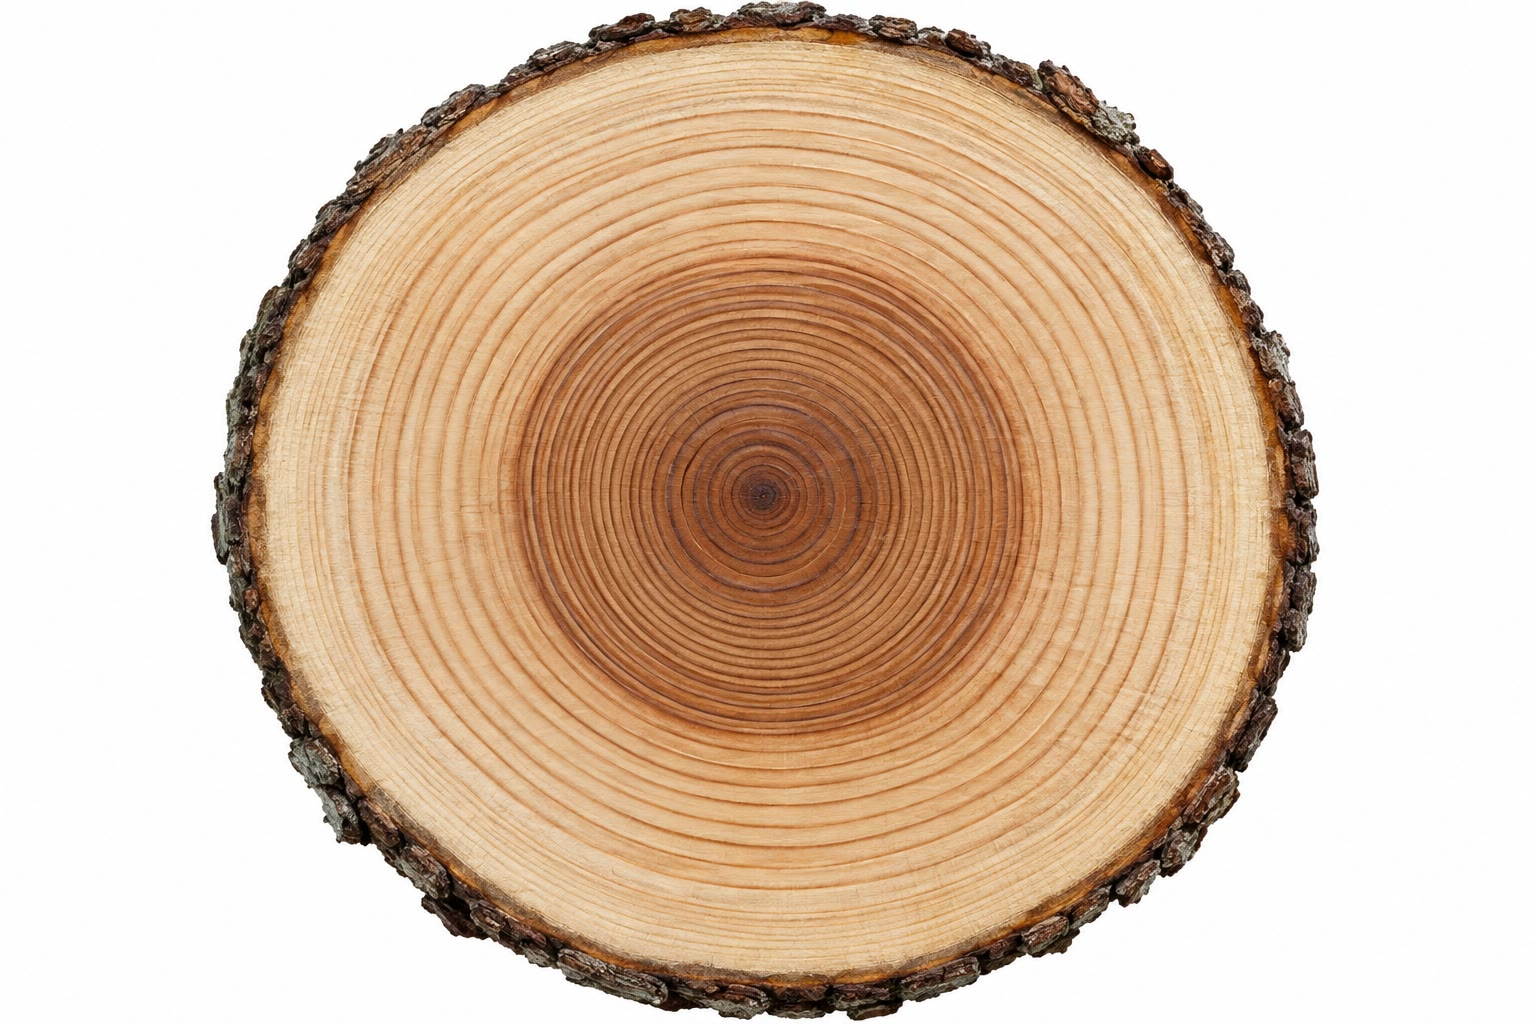
\includegraphics[width=0.5\linewidth]{images/book4/ai/b4-13-wood-rings.jpg}

{\small Um tronco de pinheiro em corte transversal: os \omterm{def:b2:plant-meristems:wood}{anéis anuais},
cada um com uma faixa clara de lenho inicial e uma faixa escura de
lenho tardio, o cerne mais escuro e a \omterm{def:b2:plant-meristems:wood}{casca}.}
\end{omfigure}

\section{Exercícios}

\begin{exercise}[$\star$]\label{exo:b2:plant-meristems:1}
Defina \omterm{def:b2:plant-meristems:meristem}{meristema} e cite os quatro \omterm{def:b2:plant-meristems:meristem}{meristemas} de uma planta lenhosa,
com o que cada um produz.
\end{exercise}

\begin{exercise}[$\star$]\label{exo:b2:plant-meristems:2}
Liste as zonas de uma ponta de raiz, da coifa para cima, com o que
acontece a uma célula em cada uma. De onde vêm as raízes laterais?
\end{exercise}

\begin{exercise}[$\star$]\label{exo:b2:plant-meristems:3}
Descreva o experimento de Thimann e Skoog, seu controle e sua
conclusão.
\end{exercise}

\begin{exercise}[$\star$]\label{exo:b2:plant-meristems:4}
Um corte de tronco mostra 60 anéis, os 15 externos claros e os demais
escuros. Dê a idade da árvore e a de seu alburno, e diga que parte do
tronco está viva.
\end{exercise}

\begin{exercise}[$\star\star$]\label{exo:b2:plant-meristems:5}
Com $\phi = \qty{0.1}{h^{-1}.MPa^{-1}}$, $Y = \qty{0.3}{MPa}$, calcule
a taxa de crescimento relativo para $P = 0.4$, $0.6$ e \qty{0.8}{MPa},
e o tempo de duplicação em cada caso. Uma seca reduz $P$ a
\qty{0.25}{MPa}: o que acontece?
\end{exercise}

\begin{exercise}[$\star\star$]\label{exo:b2:plant-meristems:6}
Folhas sucessivas surgem a \qty{137.5}{\degree} umas das outras.
Calcule as posições angulares das folhas 1 a 8 (módulo
\qty{360}{\degree}) e mostre que nenhuma das oito primeiras fica a
menos de \qty{20}{\degree} de outra. Por que isso importa para a
planta?
\end{exercise}

\begin{exercise}[$\star\star$]\label{exo:b2:plant-meristems:7}
Uma árvore de \qty{12}{m} de altura acrescenta anéis de \qty{3}{mm}.
Calcule a \omterm{def:b2:plant-meristems:wood}{madeira} acrescentada no ano em que seu raio é de
\qty{5}{cm} e no ano em que é de \qty{40}{cm}, e o carbono
correspondente (densidade seca de \qty{500}{kg/m^3}, metade carbono).
\end{exercise}

\begin{exercise}[$\star\star$]\label{exo:b2:plant-meristems:8}
Preveja os \omterm{def:b2:meiosis-heredity:vocabulary}{fenótipos} de um mutante \emph{clv3}, de um mutante
\emph{wus} e do duplo mutante, e explique a ordem dos dois genes na
alça a partir do duplo mutante.
\end{exercise}

\begin{exercise}[$\star\star$]\label{exo:b2:plant-meristems:9}
A auxina é transportada a \qty{1}{cm/h}; seu coeficiente de difusão no
tecido é \qty{1e-9}{m^2/s}. Quanto tempo o sinal leva para chegar a uma
gema \qty{20}{cm} abaixo do ápice por transporte, e por difusão
($t = x^2/2D$)? O que o transporte polar oferece à planta?
\end{exercise}

\begin{exercise}[$\star\star\star$]\label{exo:b2:plant-meristems:10}
Uma raiz de milho cresce \qty{3}{cm} por dia. As células do \omterm{def:b2:plant-meristems:meristem}{meristema}
têm \qty{20}{\micro m} de comprimento e se alongam dez vezes antes de
amadurecer; cada fileira celular tem cerca de \num{100} células em
divisão. Quantas células o \omterm{def:b2:plant-meristems:meristem}{meristema} de cada fileira precisa produzir
por dia, e que tempo de ciclo celular isso implica?
\end{exercise}

\begin{exercise}[$\star\star\star$]\label{exo:b2:plant-meristems:11}
Os trigos semianões da década de 1960 carregam \omterm{def:b2:genome-diversification:mutation}{mutações} que tornam a
planta insensível à giberelina. Explique por que eles são baixos, por
que uma planta baixa pode produzir mais grãos quando fortemente
adubada, e por que a mesma \omterm{def:b2:genome-diversification:mutation}{mutação} seria uma desvantagem numa planta
silvestre.
\end{exercise}

\begin{exercise}[$\star\star\star$]\label{exo:b2:plant-meristems:12}
``Um animal é construído uma vez; uma planta é construída a vida
inteira.'' Discuta as consequências do crescimento meristemático para a
capacidade de uma planta de responder ao ambiente, de sobreviver a
danos e de viver milênios --- e um custo dessa estratégia.
\end{exercise}

\section{Problema: Uma árvore em números}

\begin{problem}[{Problema de fim de semana --- uma árvore jovem
acompanhada durante um ano: as folhas que seu ápice produz, o
crescimento de um entrenó pela lei de Lockhart, a madeira que seu
câmbio deposita e o carbono que isso custa, e a resposta de suas gemas
à poda, até as folhas por ano, o crescimento horário do entrenó e a
madeira do ano}]
\label{pb:b2:plant-meristems:1}
Uma tília jovem tem \num{200} pontas de caule em crescimento; cada
ápice inicia uma folha a cada \num{3} dias durante uma estação de
\num{150} dias, a intervalos de \qty{137.5}{\degree}. Um entrenó em
crescimento tem \qty{2}{cm} de comprimento, e suas células têm
$\phi = \qty{0.05}{h^{-1}.MPa^{-1}}$, $Y =
\qty{0.35}{MPa}$; a turgescência é de \qty{0.55}{MPa} de dia e de
\qty{0.75}{MPa} à noite (\qty{12}{h} cada). O tronco tem \qty{8}{m} de
altura e raio de \qty{10}{cm}; o \omterm{def:b2:plant-meristems:meristem}{câmbio} acrescenta \qty{5}{mm} por ano;
a \omterm{def:b2:plant-meristems:wood}{madeira} seca tem \qty{500}{kg/m^3} e é metade carbono. A copa tem
\qty{80}{m^2} de folhas que fixam, em termos líquidos, \qty{4}{g} de
carbono por metro quadrado por dia durante \num{150} dias.

\medskip
\noindent\textbf{Parte I --- As folhas.}
\begin{enumerate}
  \item Quantas folhas um ápice produz numa estação? E a árvore
        inteira?
  \item Calcule as posições angulares das folhas 1 a 5 num caule.
  \item Após quantas folhas uma folha cai a menos de
        \qty{10}{\degree} da folha 1? (Teste múltiplos de
        \qty{137.5}{\degree}.)
  \item O que o ângulo áureo proporciona à planta, e o transporte de
        que hormônio o produz?
  \item Se cada folha tem \qty{80}{cm^2} de área, que área foliar a
        árvore constrói numa estação? Compare com os \qty{80}{m^2} que
        ela tem no meio do verão.
  \item A árvore é caducifólia. Que fração de sua área foliar ela
        reconstrói a cada primavera, e de onde vem o carbono das
        primeiras folhas?
  \item Uma \omterm{def:b2:genome-diversification:mutation}{mutação} \emph{clv3} triplica o tamanho de cada ápice. O que
        mudaria nas respostas às questões 1 e 5, e como seriam os
        caules?
\end{enumerate}

\medskip
\noindent\textbf{Parte II --- Um entrenó.}
\begin{enumerate}[resume]
  \item Calcule a taxa de crescimento relativo de dia e à noite.
  \item Calcule o comprimento acrescentado num dia e numa noite,
        partindo de \qty{2}{cm}.
  \item Ao longo de quatro desses dias, qual é o comprimento do
        entrenó? (Trate o crescimento como composto, $L(t) = L_0 e^{rt}$
        com a taxa média.)
  \item Um tratamento com giberelina reduz $Y$ a \qty{0.25}{MPa}.
        Recalcule as taxas diurna e noturna.
  \item Uma seca mantém a turgescência em \qty{0.4}{MPa} dia e noite.
        Calcule a taxa, e diga o que o ajuste osmótico faz.
  \item Explique por que o crescimento noturno supera o diurno, embora
        a fotossíntese ocorra de dia.
\end{enumerate}

\medskip
\noindent\textbf{Parte III --- A \omterm{def:b2:plant-meristems:wood}{madeira}.}
\begin{enumerate}[resume]
  \item Calcule o volume de \omterm{def:b2:plant-meristems:wood}{madeira} acrescentado neste ano e sua massa
        seca.
  \item Calcule o carbono que ela contém.
  \item Calcule o carbono fixado pela copa ao longo da estação.
  \item Que fração do carbono da copa foi para a \omterm{def:b2:plant-meristems:wood}{madeira} do tronco? Cite
        três outros drenos.
  \item Em vinte anos, com a mesma largura de anel, qual será o
        incremento anual de \omterm{def:b2:plant-meristems:wood}{madeira}? Por que ele aumenta?
  \item Dois anéis do tronco têm metade da largura de seus vizinhos.
        Sugira duas causas e diga como um dendrocronologista as
        distinguiria.
\end{enumerate}

\medskip
\noindent\textbf{Parte IV --- Gemas e poda.}
\begin{enumerate}[resume]
  \item O jardineiro corta todas as pontas dos caules. Preveja a
        resposta das gemas axilares e a forma da árvore em um mês.
  \item Como uma pasta de auxina aplicada em cada corte alteraria a
        resposta?
  \item Uma sebe é aparada seis vezes por ano. Explique, com a
        \omterm{prop:b2:plant-meristems:apical}{dominância apical}, por que ela fica densa.
  \item Uma árvore cortada rente ao solo rebrota uma dúzia de caules. De
        onde eles vêm, e por que uma planta sobrevive à perda de todos
        os caules, quando um animal não sobrevive à perda da cabeça?
  \item A citocinina das raízes sobe depois que as raízes são regadas.
        Preveja o efeito sobre a brotação das gemas.
  \item Enuncie o resultado: folhas por ápice e por árvore por estação,
        as taxas de crescimento diurna e noturna do entrenó, e a \omterm{def:b2:plant-meristems:wood}{madeira}
        e o carbono do ano.
\end{enumerate}
\end{problem}
